%!TEX root = bachelor.tex
\chapter{Methodik}
\label{ch:method}

In diesem Kapitel stellen wir ein Verfahren vor, dass ermöglicht anhand eines Bildes (siehe Einleitung).

Zunächst gehen wir auf das verwendete Kalibrierungsmuster ein, woraufhin die genaue Vorgehensweise zur Entfaltung erläutert wird. 

Die geometrischen Eigenschaften des Kegelstumpfs $(r, R, \Delta H)$ können gemessen und somit als bekannt angenommen werden. 
Darüber hinaus nehmen wir an, dass sich das Zentrum des kleineren Kreises im links-händigen Weltkoordinatensystem an der Positon $(0,0,0)$ (siehe Abbildung \ref{fig:coneFrustum}) befindet. Durch diese Einschränkung gehen jegliche absolute Größenverhältnisse verloren. Es ist also nicht mehr möglich die Größe einer Larve zu bestimmen. 

Wir wollen eine Beziehung zwischen Bildpunkte und Kegelpunkten herstellen. wo ist z achse?


\section{Kalibrierungsmuster}
\label{s:calibrationPattern}
Um eine Beziehung zwischen Bildpunkten und Kegelpunkten herstellen zu können, ist ein Kalibrierungsmuster notwendig.

Die Wahl des Kalibrierungsmusters spielt dabei eine entscheidende Rolle bei der Robustheit und Präzision der Entfaltung. Es muss gewährleistet sein, dass die charakteristischen Merkmale des Musters, auch bei leichten Abweichungen der Kamera vom Lot und schlechteren Beleuchtungssituationen zuverlässig erkannt werden. Das Muster muss darüber hinaus so entworfen sein, dass beim zusammenlegen im Kegel, dessen geometrische Eigenschaften nicht verfälscht, sondern realitätsgetreu wiedergeben werden. 

Wir haben uns für ein Muster entscheiden, dass in äquidistanten Abständen $\Delta R$, beginnend mit dem kleinen Radius $r$ des Kegelstumpfs (siehe Abbildung \ref{fig:coneFrustum}) Kreislinien und in gleichen Winkelabständen $\Delta \alpha$ auf der Seitenhöhe Liniensegmente besitzt. Das zusammengelegte Muster ist in Abbildung \ref{fig:calibrationPatternTop} zu sehen, beziehungsweise das entfaltete in \ref{fig:calibrationPattern}. Die Anzahl der Kreislinien wird mit $n$ gekennzeichnet, die Anzahl sichtbarer Liniensegmente im Kegel mit $m$. Zu beachten ist, dass bedingt durch das Entfalten, in \ref{fig:calibrationPattern}  ein Liniensegment doppelt zu sehen ist. Die schwarzen Kreise bezeichnen wir als Samples. 

Dadurch dass die Geometrie des Kegels bekannt ist, kann jedem Sample nun ein Punkt auf dem Kegel im Weltkoordinatensystem zugeordnet werden. Da ein Kegel beliebig um die $Y$ Achse rotiert werden, kann ist diese Abbildung zunächst nicht eindeutig. Dazu nehmen wir an, dass das Liniensegment mit dem kleinsten Winkel zur $X$-Achse mit dem Kegelwinkel $\theta = 0$ korrespondiert (siehe \ref{eq:paramFrustum}).

\begin{figure}[!htb]
	\centering
	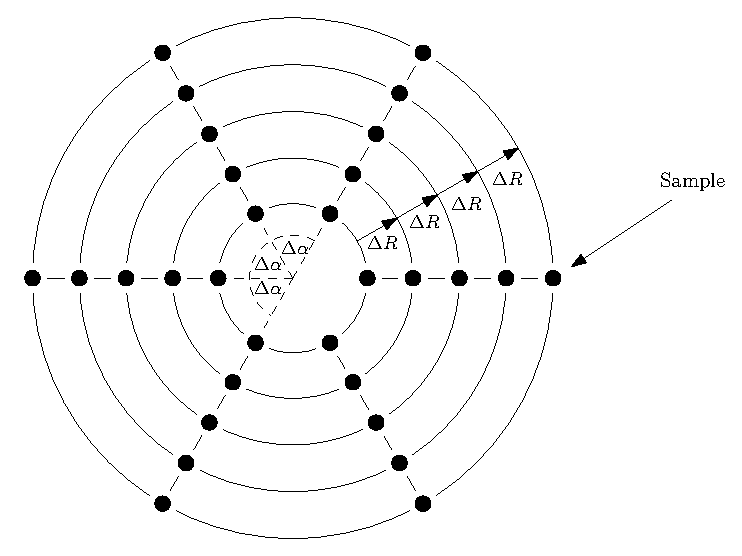
\includegraphics[scale=.8]{images/calibrationPatternTop.eps}
	\caption{Kalibrierungsmuster von oben mit $n = 5, m = 6$}
	\label{fig:calibrationPatternTop}
\end{figure}


\begin{figure}[!htb]
	\centering
	\includegraphics[scale=.7]{images/calibrationPattern2.eps}
	\caption{Kalibrierungsmuster entfaltet mit $n = 5, m = 6$}
	\label{fig:calibrationPattern}
\end{figure}

Das Muster ist also 

\subsection{Anzahl der Samples}
Die Anzahl der Samples sollte groß genug sein, um möglichst viel geometrische Informationen des Kegels zu erhalten, aber klein genug, dass eine Detektion der Samples problemlos möglich ist. Insbesondere auf dem innersten Kreis, macht sich eine zu hohe Sampleanzahl negativ bemerkbar, da der Abstand zueinander sehr klein wird, was eine Detektion erschwert. Des Weiteren sollte noch ein möglichst großer Teil der Kreislinie zu sehen bleiben, da diese für die Ellipsendetektion benötigt werden \todo{siehe später, dazu mehr später????}


\todo{warum gerade dieses muster? warum ist das so gut? wie berechnet man das muster? welche eigenschaften hat es?}


Bilder von kegel mit muster drin?

\section{Intrinsische Kamerakalibrierung}

Bedingt durch die Wahl einer Weitwinkelkamera, enthält die Linse der Kamera eine starke tonnenförmige (nach außen gewölbte) Verzerrung. Ohne eine intrinsische Kamerakalibrierung würde. Es werden nur die intrinsischen Parameter benötigt. \todo{ Warum die extrinsciehn nicht? kamera postion gegeben dann ??}

\todo{Vergleich ohne und mit Kalibrierung}

\begin{figure}[!htb]
	\centering
\begin{subfigure}{.5\textwidth}
	\centering
	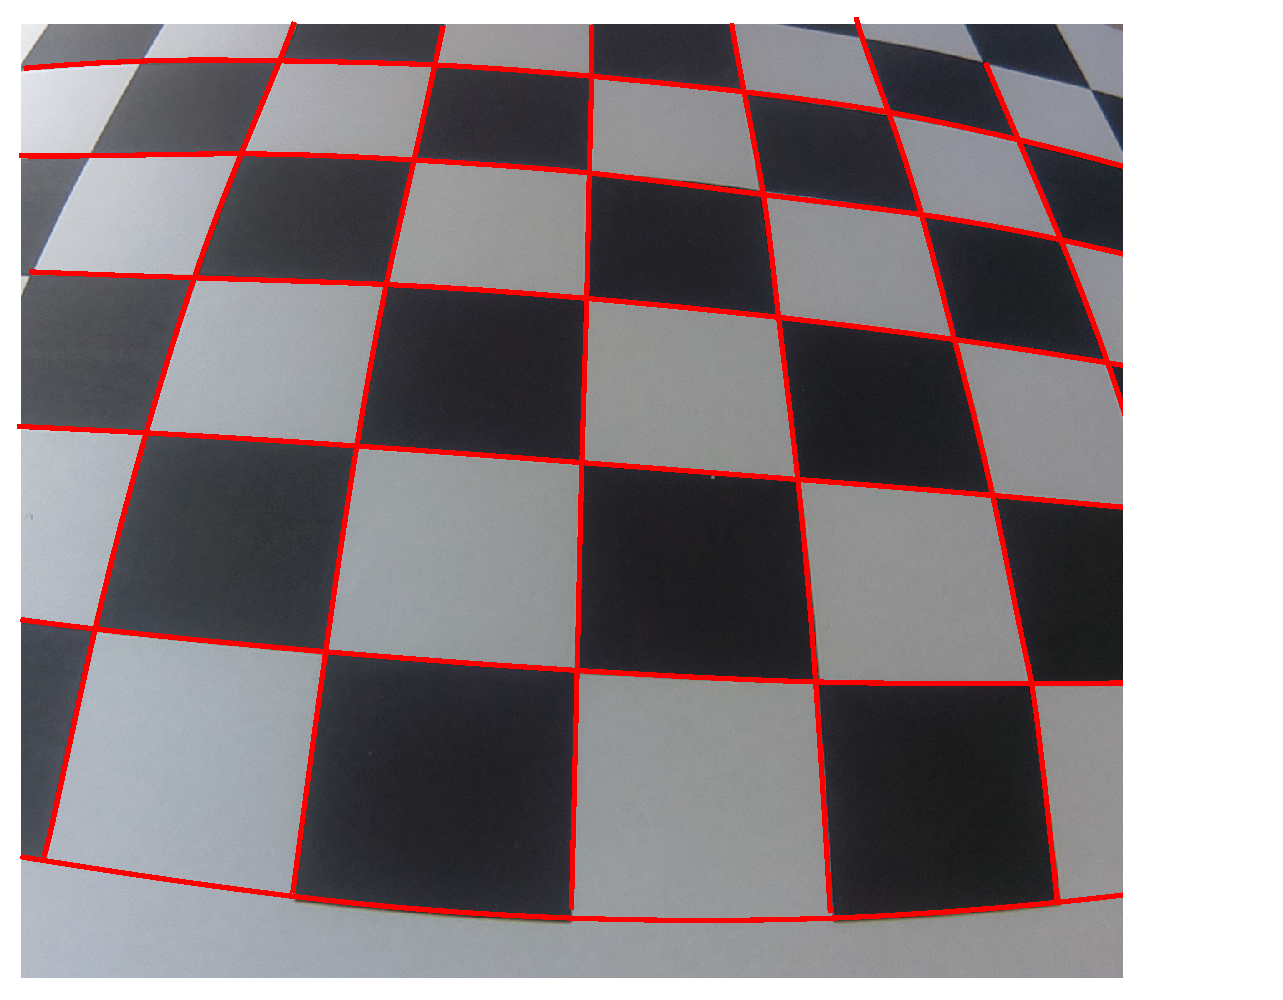
\includegraphics[scale=.35]{images/calibrationRaspi.eps}
	\caption{vor Kalibrierung}
	\label{fig:calibDist}
\end{subfigure}%
\begin{subfigure}{.5\textwidth}
	\centering
	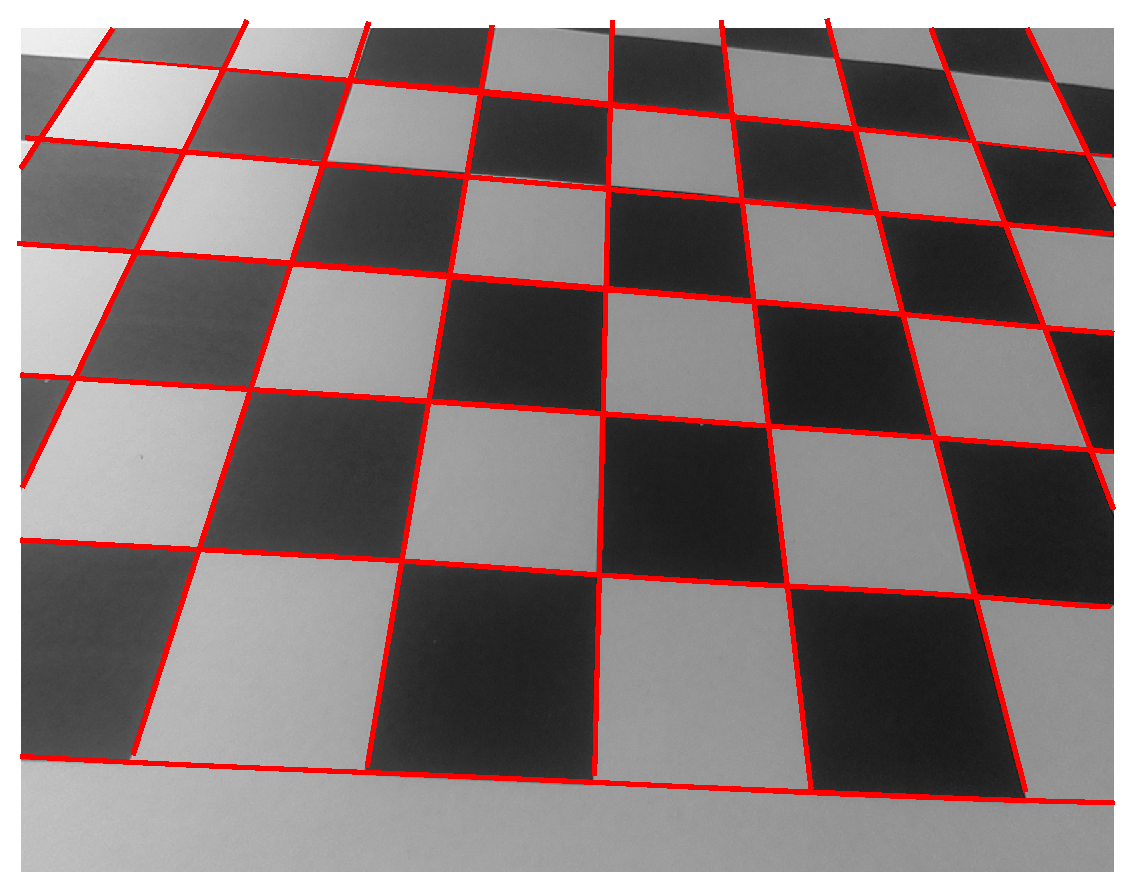
\includegraphics[scale=.4]{images/calibrationRaspi2.eps}
	\caption{nach Kalibrierung und Entzerrung}
	\label{fig:calibUndist}
\end{subfigure}
\caption{Kamerakalibrierung}
\label{fig:calib}
\end{figure}


\section{Detektion der Samples} \todo{Umbennenen}

Nach der Kamerakalibrierung und entsprechender Entzerrung werden die Bildkoordinaten der Samples bestimmt. Dazu ist wird ein Blob-Detektor \ref{s:blob} benutzt. Um die Samples korrekt von den Kreislinien, sowie den Liniensegmenten trennen zu können, ist es wichtig dass die Umgebung eines Samples frei ist. \todo{Formulierung}.

Filtert Farbe (schwarz), kleine Flächen werden verworfen, Kreisförmigkeit, Konvexität

\section{Ellipsen-Detektion}
Nachdem die Samplepositionen bestimmt wurden, muss für jeden Sample entschieden werden, auf welcher der Kreislinien er liegt. Da die Kreise, bedingt durch perspektivische Verzerrung, zu  Ellipsen werden, wird eine Verfahren 
benötigt, dass Ellipsen erkennt. 

Zunächst werden die Kanten mit Hilfe von Canny (\ref{s:canny}) detektiert (siehe Abbildung \ref{fig:canny}). 

\begin{figure}[!htb]
	\centering
	\begin{subfigure}{.5\textwidth}
		\centering
		\includegraphics[scale=.2]{images/grey.png}
		\caption{Grauwertbild}
		\label{fig:beforeCanny}
	\end{subfigure}%
	\begin{subfigure}{.5\textwidth}
		\centering
		\includegraphics[scale=.2]{images/canny.png}
		\caption{Canny-Kanten}
		\label{fig:afterCanny}
	\end{subfigure}
	\caption{Canny-Kantendetektion auf Grauwertbild}
	\label{fig:canny}
\end{figure}

Anschließend versuchen wir möglichst genau das Zentrum der innersten Ellipsen zu bestimmen.
Wir benutzen dafür Hough-Transformationen, um Linien im Canny-Bild zu \todo{hier passendes Wort einfügen}.
Es werden anschließend Schnittpunkte aller Liniensegmente bestimmt. Bedingt durch Ungenauigkeiten beim Ausschneiden und Zusammenlegen im Kegel, schneiden sich nicht alle Liniensegmente in einem Punkt.
Darüber hinaus werden, auf Grund der Liniendicke auf dem Kalibrierungsmuster, durch Canny viele Linien doppelt erkannt. Auch ein inhomogener Hintergrund, erschwert die Schnittpunktsbestimmung. Um also möglichst robust einen Kandidaten auszuwählen, wird zuerst der Median der $x$-Koordinaten der Schnittpunkte und dann der Median der $y$-Koordinaten bestimmt. Die erhaltenen Koordinaten bilden den Schnittpunkt (siehe Abbildung \ref{fig:houghLines}).

Von diesem Schnittpunkt aus werden, in einer vorher definierte Anzahl, gleichmäßig, in alle Richtungen Strahlen ausgesendet. \todo{Komma-Setzung}. 
Trifft ein Strahl ein weißes Pixel, wird dessen Position gekennzeichnet, trifft er den Rand des Bildes, wird er ignoriert. 

\begin{figure}[!htb]
	\centering
	\includegraphics[scale=.25]{images/houghLines.png}
	\caption{Hough-Transformation zur Linien-Detektion (in rot gekennzeichnet) und bestimmter Schnittpunkt (in grün) }
	\label{fig:houghLines}
\end{figure}

warum sollte das robust sein? siehe raycast
ransac anzahl iterationen: großzügig da laufzeit unwichtig

\newpage
\section{Zuordnung der Punkte}
nach winkel sortieren und dann kürzeste distanz

ellipsen neuschätzen
dann geraden durch ziehen

\section{Weltkoordinaten bestimmen}

\section{Entfaltung}
\subsection{Vorwärts}
\begin{figure}[!htb]
	\centering
	\includegraphics[scale=.6]{images/radialInterpolation.eps}
	\caption{Interpolation}
	\label{fig:Interpolation}
\end{figure}
\subsection{Rückwärts}
Projektionsmatrix bestimmen
